\documentclass{article}
\usepackage{authblk}
\usepackage{titling}
\usepackage{graphicx}
\usepackage{wrapfig}
\usepackage{subfig}
\usepackage{float}

\title{Urban Heat Islands in Mid-Sized Cities}
\author[1]{Omar Haddad}
\author[1,2]{Lena Fischer\thanks{Corresponding author: lena@example.de}}
\author[2]{Raj Kumar}
\affil[1]{Department of Geography, University A}
\affil[2]{Institute for Climate, University B}
\renewcommand\Authands{ and }
\predate{}
\postdate{}
\date{}
\pretitle{\begin{center}\LARGE\bfseries}
\posttitle{\end{center}}

\begin{document}
\maketitle

\section{Study area}
\begin{wrapfigure}{r}{0.4\textwidth}
  \centering
  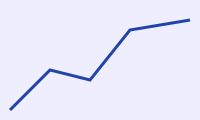
\includegraphics[width=0.38\textwidth]{plot.svg}
  \caption{Temperature anomaly.}
  \label{fig:anom}
\end{wrapfigure}
The cities studied range from 100{,}000 to 500{,}000 inhabitants. Figure~\ref{fig:anom} shows the anomaly.

\begin{figure}[H]
  \centering
  \subfloat[Summer\label{fig:summer}]{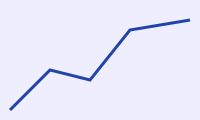
\includegraphics[width=0.45\textwidth]{plot.svg}}
  \hfill
  \subfloat[Winter\label{fig:winter}]{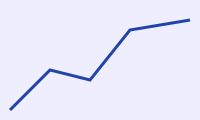
\includegraphics[width=0.45\textwidth]{diagram.svg}}
  \caption{Seasonal patterns.}
  \label{fig:seasons}
\end{figure}

Figures~\ref{fig:summer} and~\ref{fig:winter}.

\begin{figure}[ht]
\centering
\scalebox{0.5}{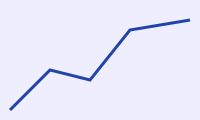
\includegraphics{plot.svg}}
\rotatebox{90}{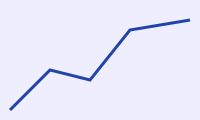
\includegraphics[height=2cm]{diagram.svg}}
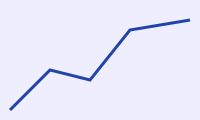
\includegraphics[scale=0.3, angle=0, trim=0 0 0 0, clip]{plot.svg}
\caption[Short caption]{Transformed images with a long caption.}
\end{figure}
\end{document}
